\newpage
\subsection{Goal}

Experimental study of the time complexity of different algorithms.

\subsection{Formulation of the problem}

For each n from 1 to 2000, measure the average computer execution time of programs implementing the algorithms and functions below for five runs.
Plot the data obtained showing the average execution time as a function of n. Conduct the theoretical analysis of the time complexity of the algorithms in question and compare the empirical and theoretical time complexities.

\paragraph{I.}
Generate an $n$-dimensional random vector $v=[v_1,v_2,...,v_n]$ with non-negative elements.
For $v$, implement the following calculations and algorithms:
\begin{itemize}
    \item $f(v) = const$ (constant function);
    \item $f(v) = \sum^{n}_{k = 1}{v_k}$ (the sum of elements);
    \item $f(v) = \prod^{n}_{k = 1}{v_k}$ (the product of elements);
    \item supposing that the elements of $v$ are the coefficients of a polynomial $P$ of degree $n - 1$, calculate the value $P(1.5)$ by a direct calculation of $P(x) = \sum^{n}_{k = 1}{v_kx^{k - 1}}$ (i.e. evaluating each term one by one) and by Horner's method by representing the polynomial as $P(x) = v_1 + x(v_2 + x(v_3 + ...))$;
    \item Bubble Sort of the elements of $v$;
    \item Quick Sort of the elements of $v$;
    \item Timsort of the elements of $v$.
\end{itemize}

\paragraph{II.}
Generate random matrices $A$ and $B$ of size $n \times n$ with non-negative elements. Find the usual matrix product for $A$ and $B$.

\paragraph{III.}
Describe the data structures and design techniques used within the algorithms.

\subsection{Brief theoretical part}

Time complexity is characteristic of algorithm, which provides information about the amount of time necessary to process given amount of data.

The time complexity of the algorithm is estimated by counting the number of elementary operations (addition, multiplication, etc.) performed by the algorithm for a given amount of data. It is assumed that each elementary operation requires a fixed amount of time.

A \textbf{constant function}, \textbf{the sum of elements}, \textbf{the product of elements}, and \textbf{the calculation of the polynomial} are calculated in a single pass through the loop.
They use an iterative strategy.

\textbf{Bubble sort} is a simple sorting algorithm.
This sorting algorithm is comparison-based algorithm in which each pair of adjacent elements is compared and the elements are swapped if they are not in order.
An iterative pattern is also used here.

\textbf{Quick Sort} is a sorting algorithm, which is commonly used in computer science.
Quick Sort is a divide and conquer algorithm.
It creates two empty arrays to hold elements less than the pivot value and elements greater than the pivot value, and then recursively sort the sub arrays.
There are two basic operations in the algorithm, swapping items in place and partitioning a section of the array.

\textbf{TimSort} is a stable, adaptive iterative merge sort that requires a small number of comparisons when working with partially sorted arrays, while providing performance comparable to traditional merge sorting when working with random arrays.

\subsection{Results}

\paragraph{Constant function $f(v) = 1$.}

With the exception of one peak, which is related to the computing platform, the theoretical and empirical estimates are the same - $O(1)$ (Figure \ref{ris:constant_function}).

\begin{figure}[H]
    \center
    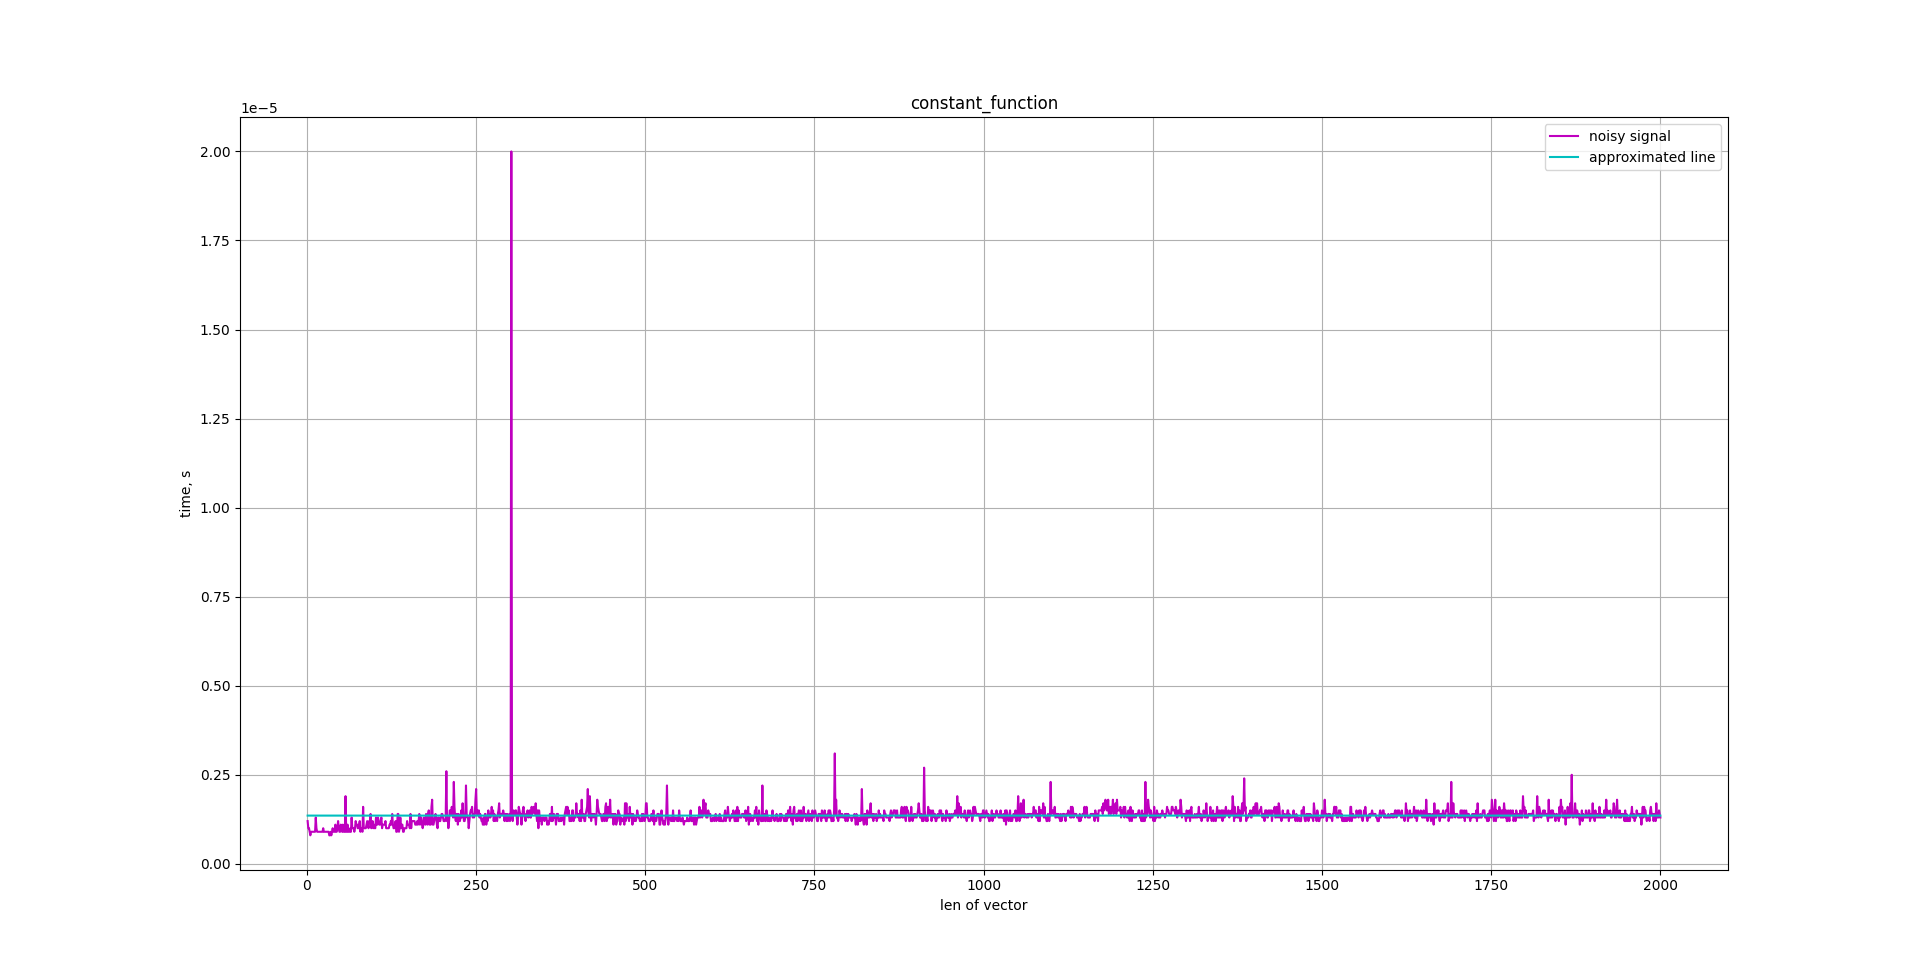
\includegraphics[width=\textwidth]{img/constant_function.png}
    \caption{Empirical and theoretical time complexities of an algorithm that implements the function $f(v) = \sum^{n}_{k = 1}{v_k}$.}
    \label{ris:constant_function}
\end{figure}

\paragraph{Sum and product of elements.}

Despite the $y$-axis spikes, these functions are approximated by a straight line and coincide with the theoretical estimate - $O(n)$ (Figure \ref{ris:sum_function}, \ref{ris:prod_function}).

\begin{figure}[H]
    \center
    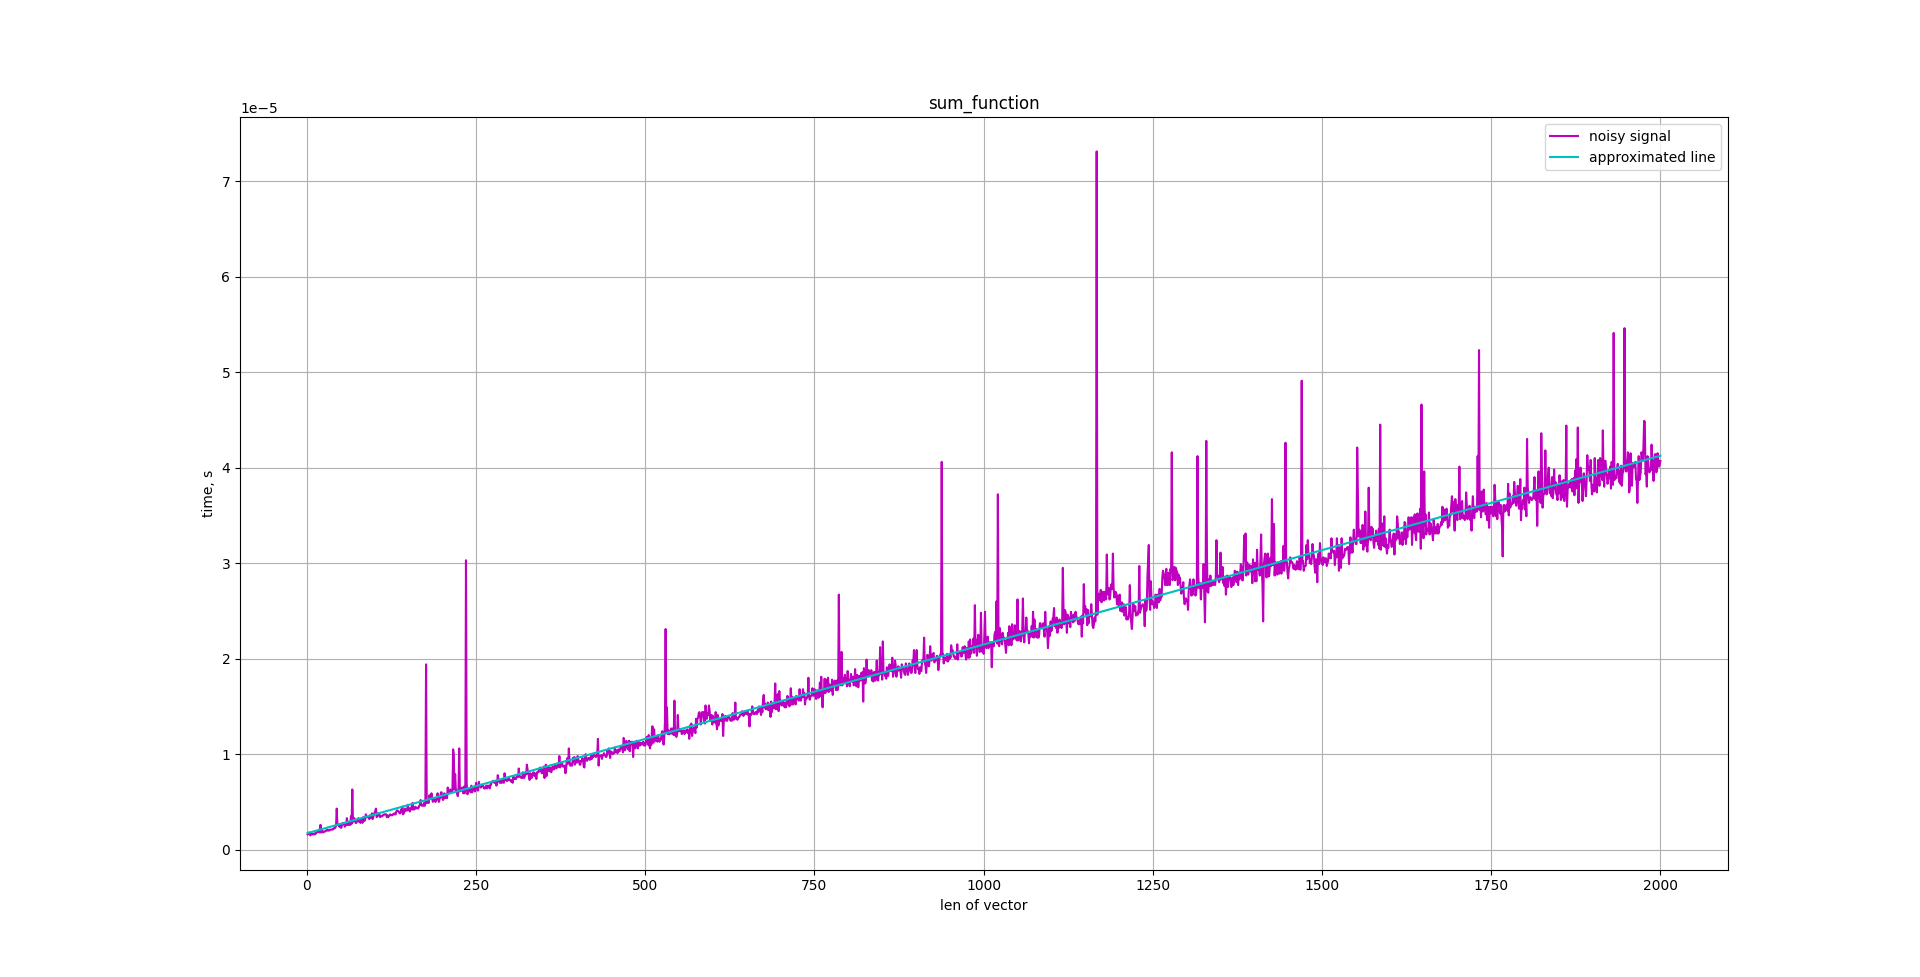
\includegraphics[width=\textwidth]{img/sum_function.png}
    \caption{Empirical and theoretical time complexities of an algorithm that implements the function $f(v) = \prod^{n}_{k = 1}{v_k}$.}
    \label{ris:sum_function}
\end{figure}

\begin{figure}[H]
    \center
    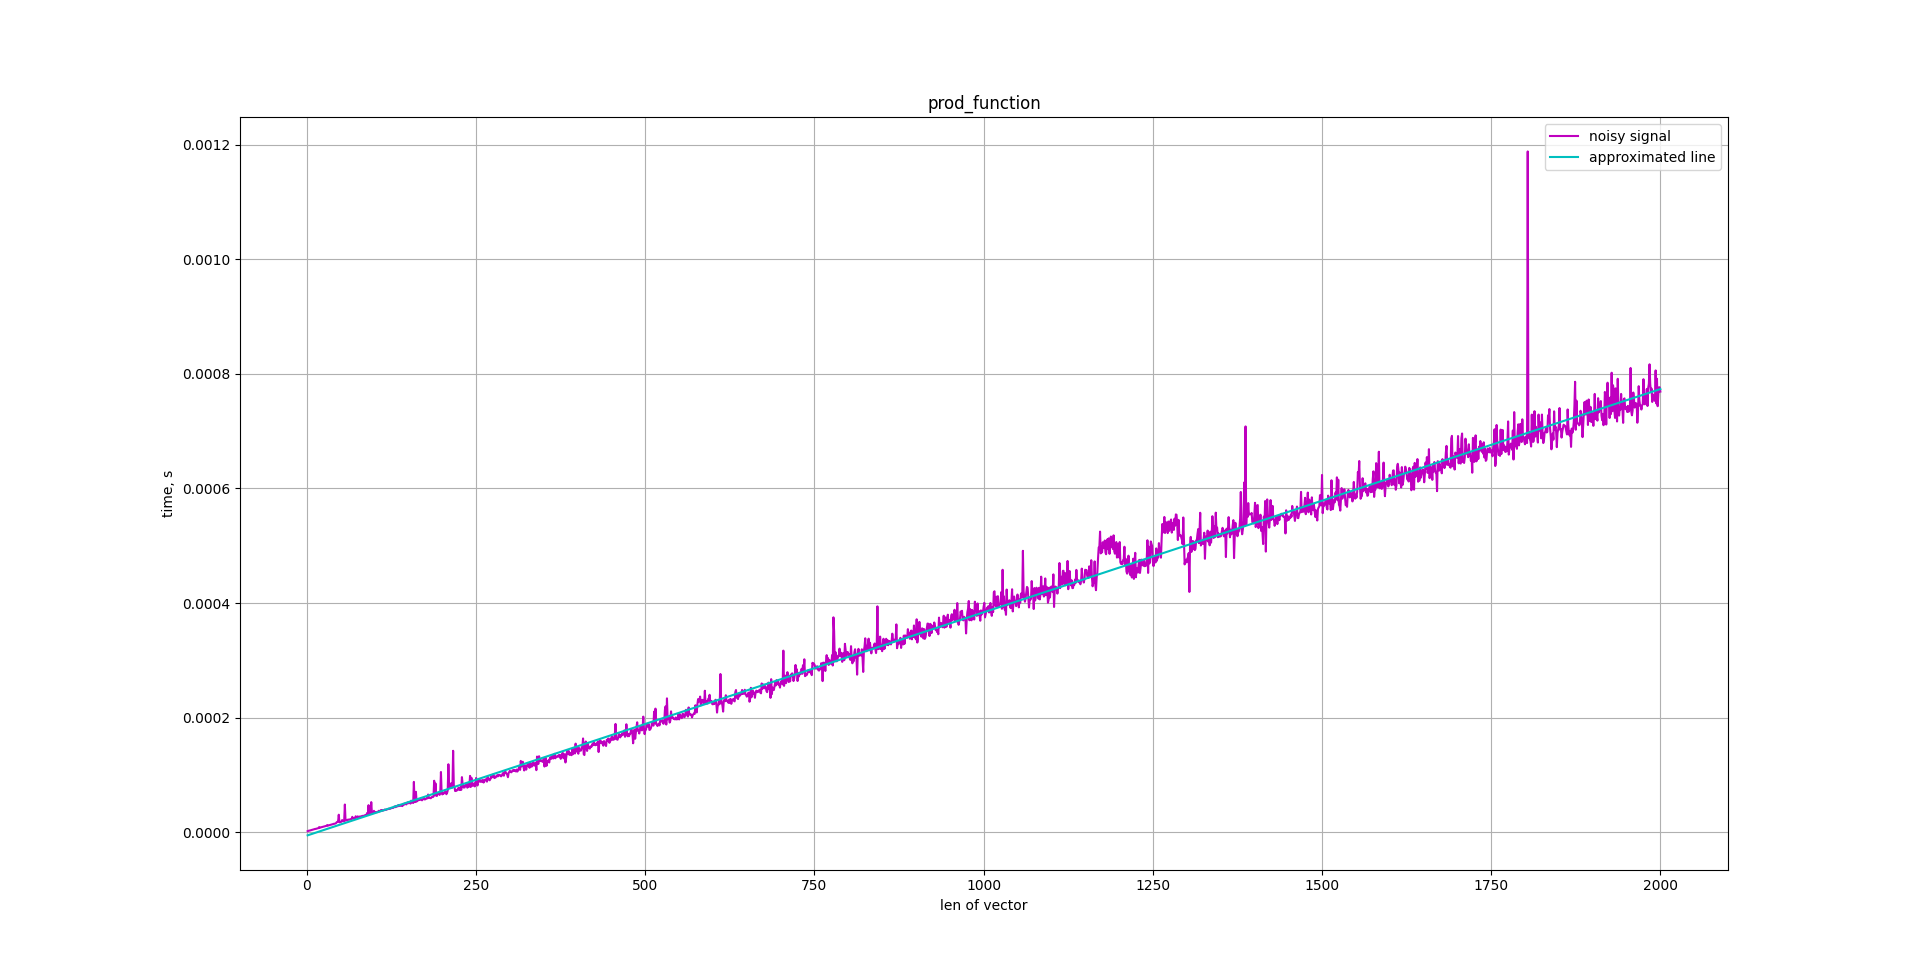
\includegraphics[width=\textwidth]{img/prod_function.png}
    \caption{Empirical and theoretical time complexities of an algorithm that implements the function $P(x) = \sum^{n}_{k = 1}{v_kx^{k - 1}}$.}
    \label{ris:prod_function}
\end{figure}

\paragraph{Calculation of the polynomial.}

The direct calculation and the Horner's method also correspond to the theoretical estimate - $O(n)$ (Figure \ref{ris:naive_poly_function}, \ref{ris:horner_method_function}). It is worth noting that the result, when calculated directly, despite the use of long arithmetic, overflows the buffer when the length of vector is $>1750$.

\begin{figure}[H]
    \center
    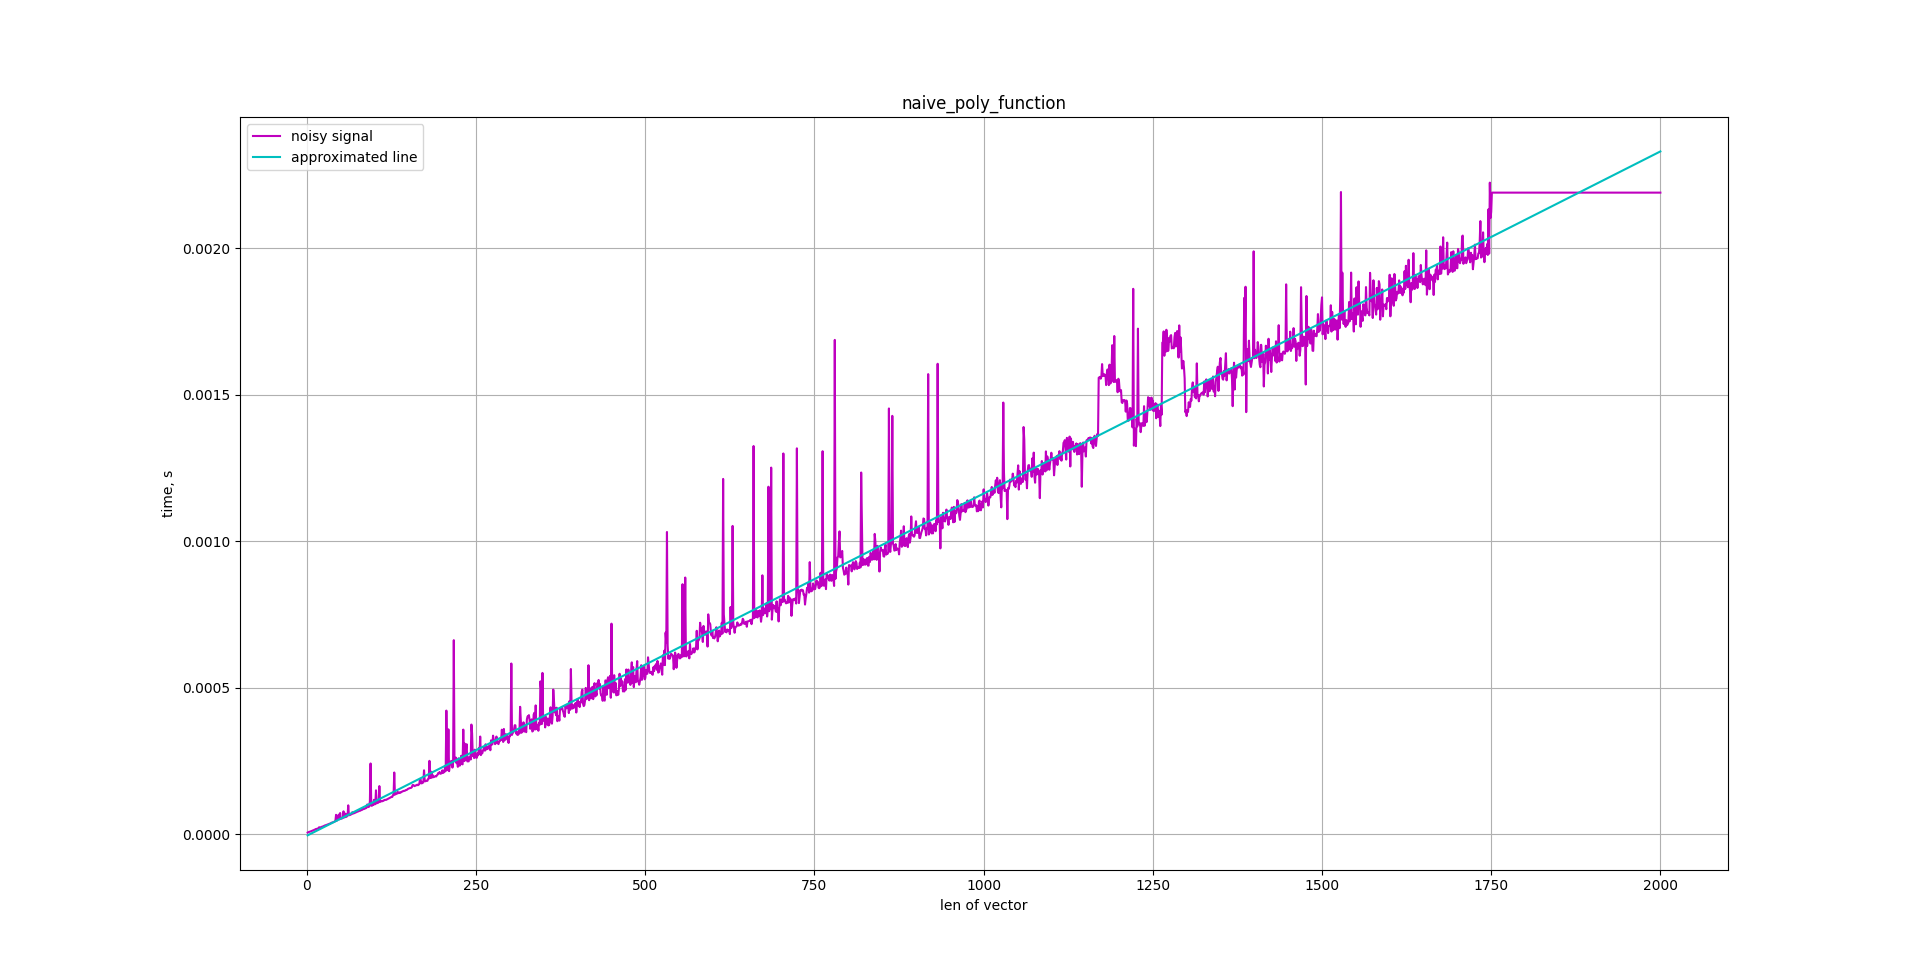
\includegraphics[width=\textwidth]{img/naive_poly_function.png}
    \caption{Empirical and theoretical time complexities of an algorithm that
implements the function $P(x) = \sum^{n}_{k = 1}{v_kx^{k - 1}}$.}
    \label{ris:naive_poly_function}
\end{figure}

\begin{figure}[H]
    \center
    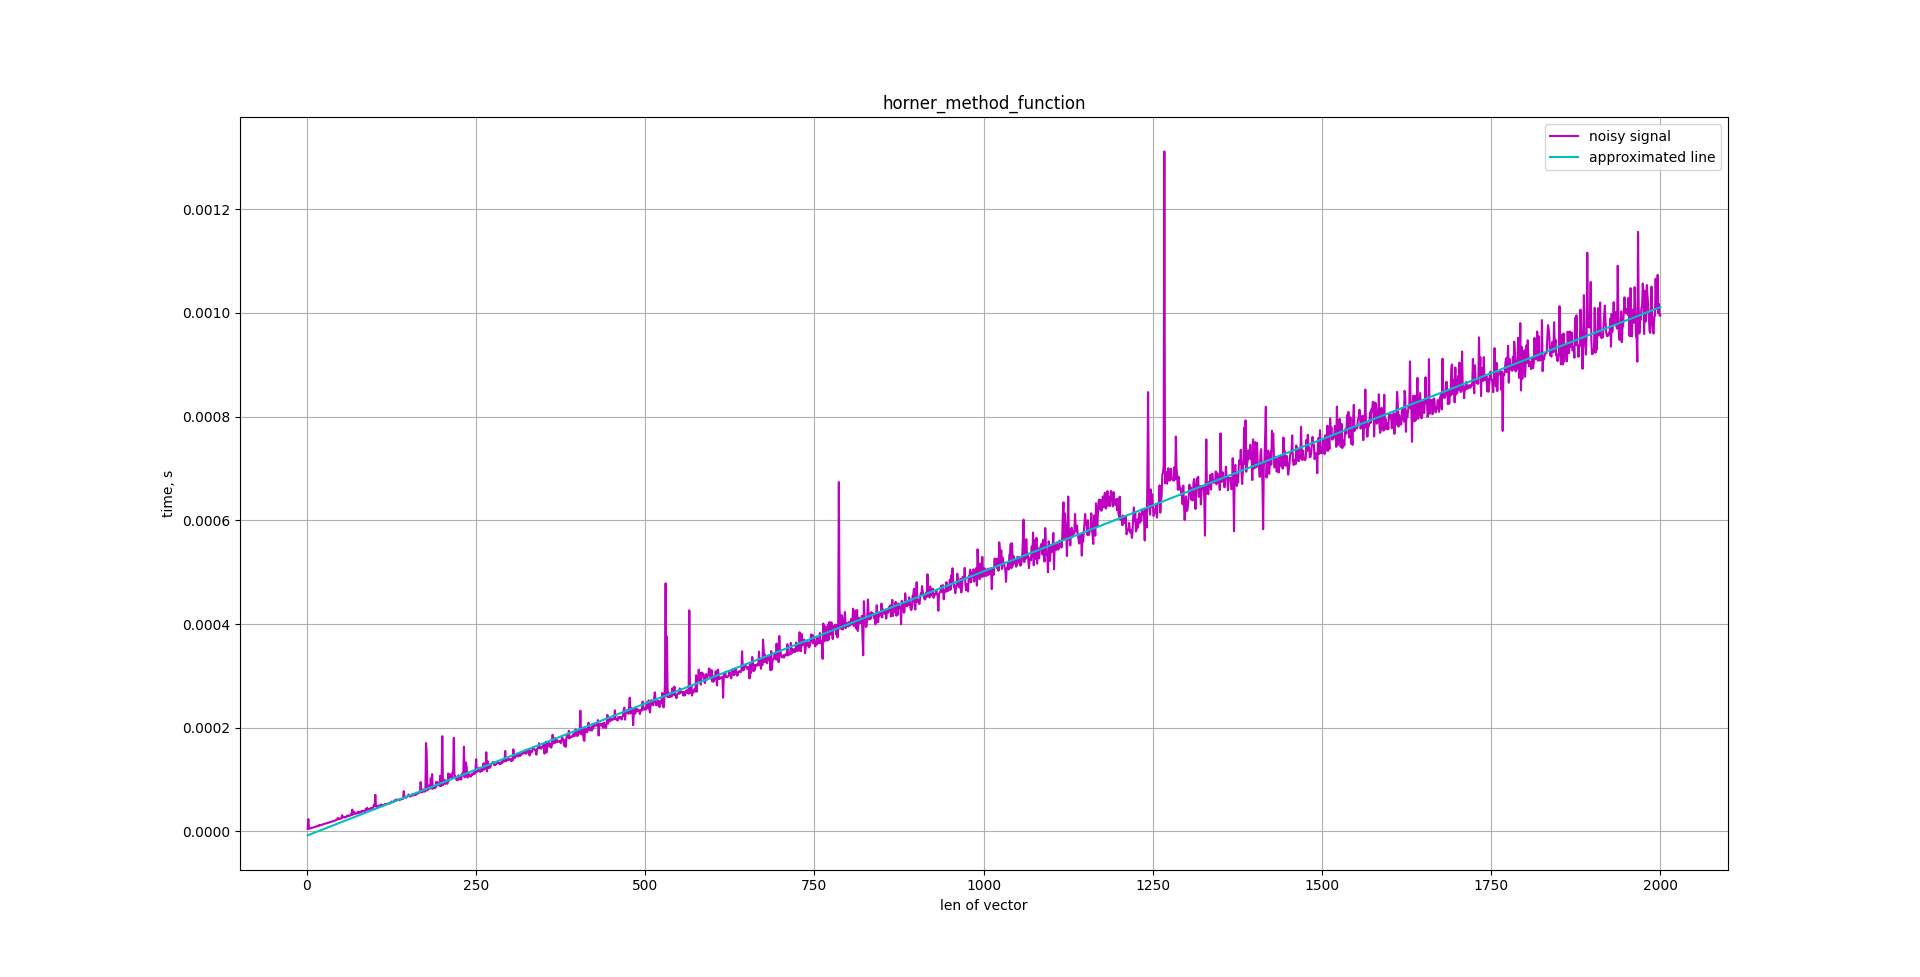
\includegraphics[width=\textwidth]{img/horner_method_function.png}
    \caption{Empirical and theoretical time complexities of an algorithm that implements the function $P(x) = v_1 + x(v_2 + x(v_3 + ...))$.}
    \label{ris:horner_method_function}
\end{figure}

\paragraph{Bubble Sort.}

Bubble sorting has an average time complexity of $O(n^2)$, which is shown on Figure \ref{ris:bubble_sort}.

\begin{figure}[H]
    \center
    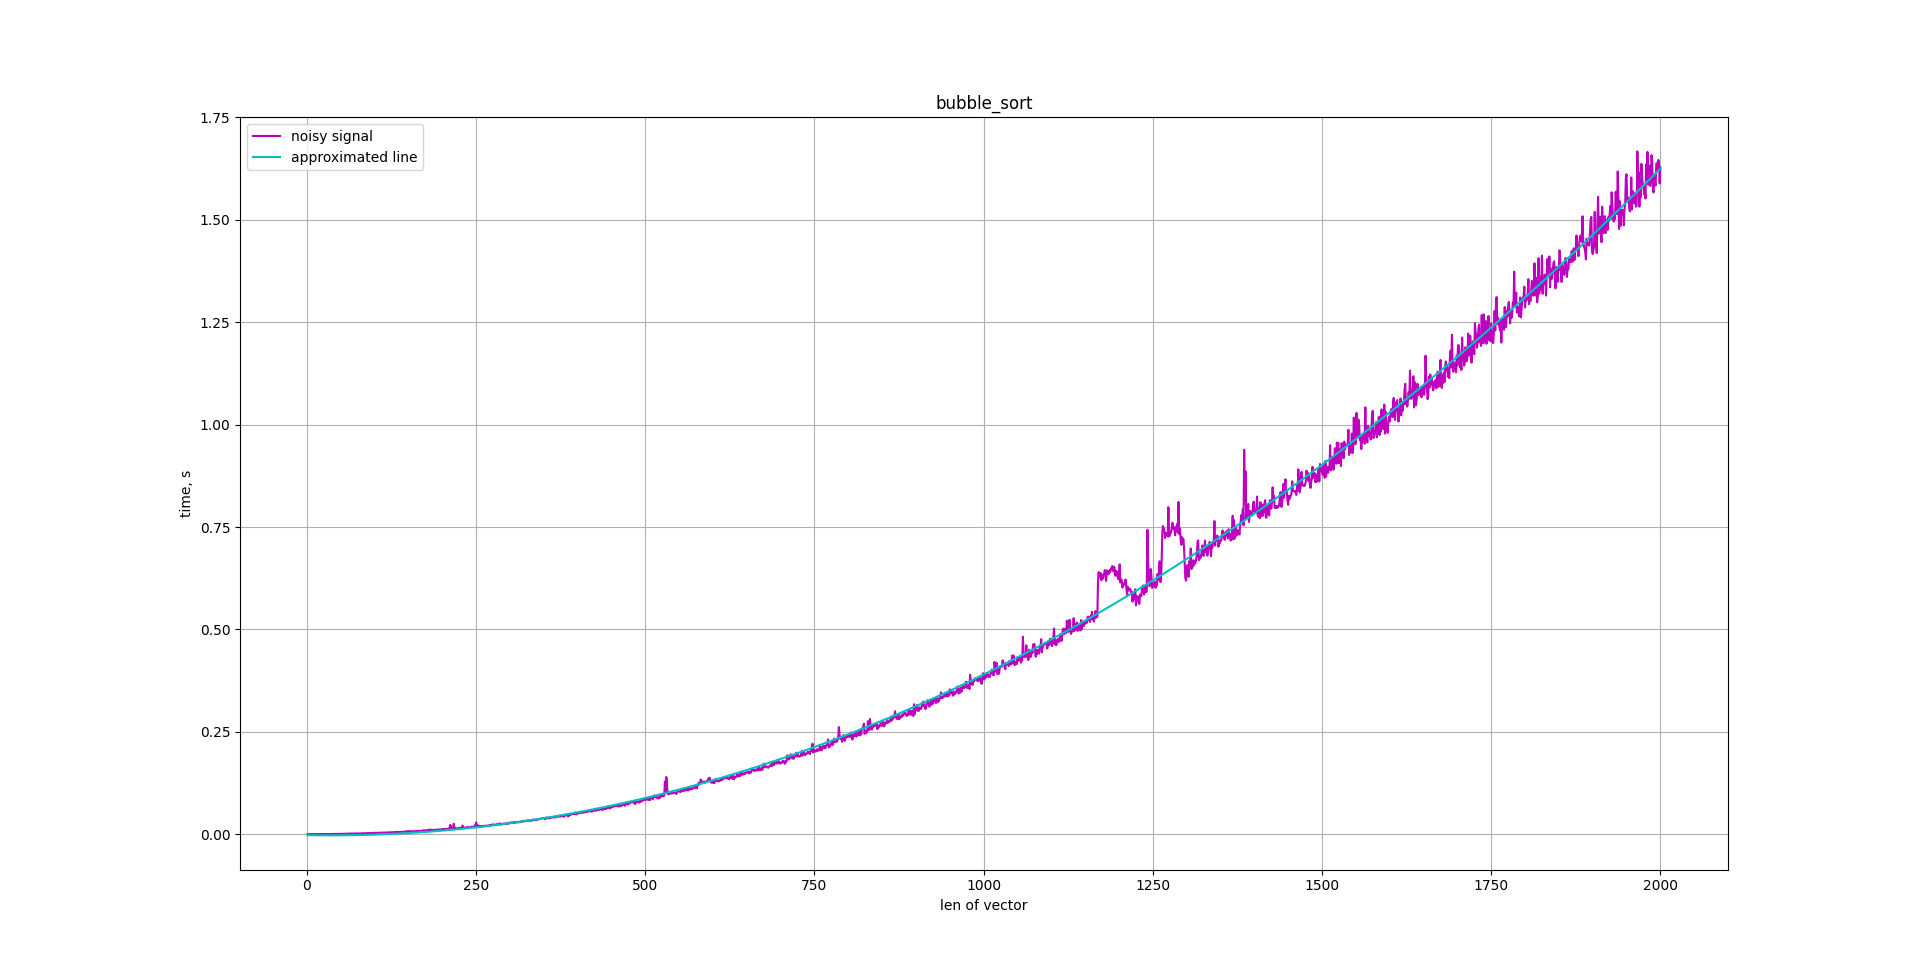
\includegraphics[width=\textwidth]{img/bubble_sort.png}
    \caption{Empirical and theoretical time complexities of an algorithm that implements the Bubble Sort.}
    \label{ris:bubble_sort}
\end{figure}

\paragraph{Quick Sort and TimSort.}

Quick sort and Timsort in the average case have a theoretical complexity of $O(n\log{n})$ and are approximated by linear functions . This is confirmed by an empirical experiment (Figure \ref{ris:quick_sort}, \ref{ris:timsort}).

\begin{figure}[H]
    \center
    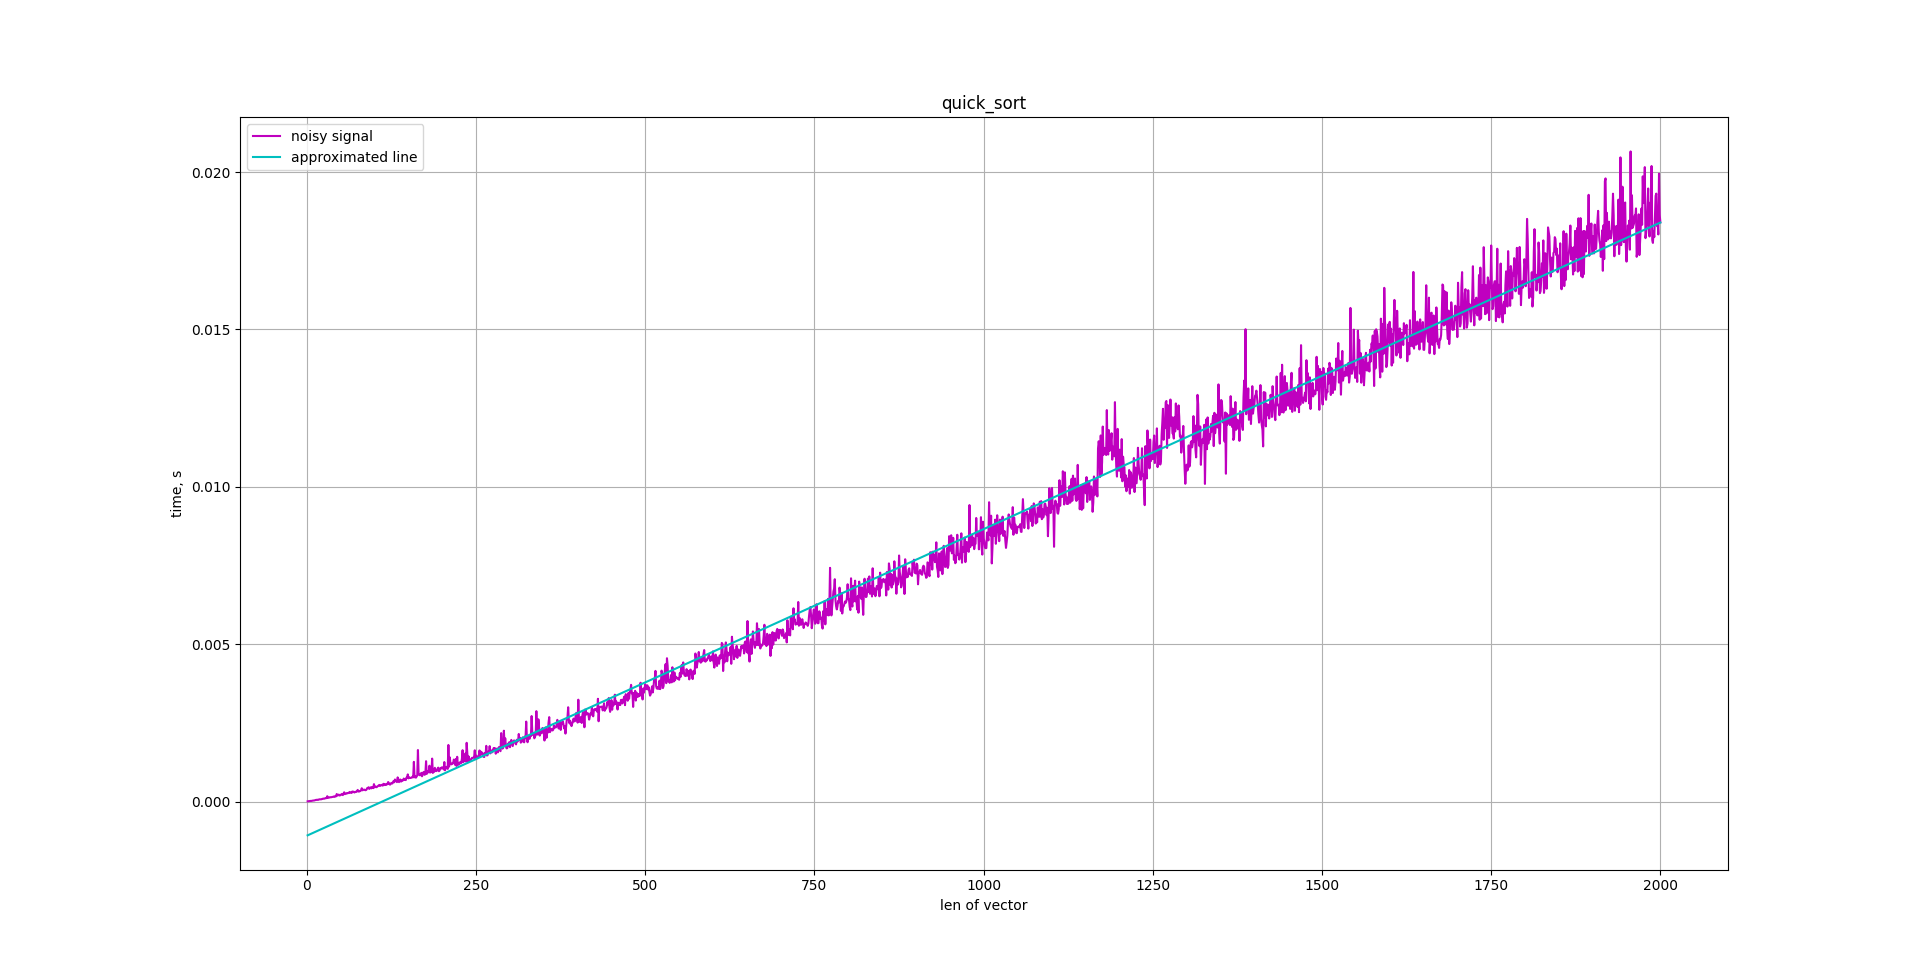
\includegraphics[width=\textwidth]{img/quick_sort.png}
    \caption{Empirical and theoretical time complexities of an algorithm that
implements the Quick Sort.}
    \label{ris:quick_sort}
\end{figure}

\begin{figure}[H]
    \center
    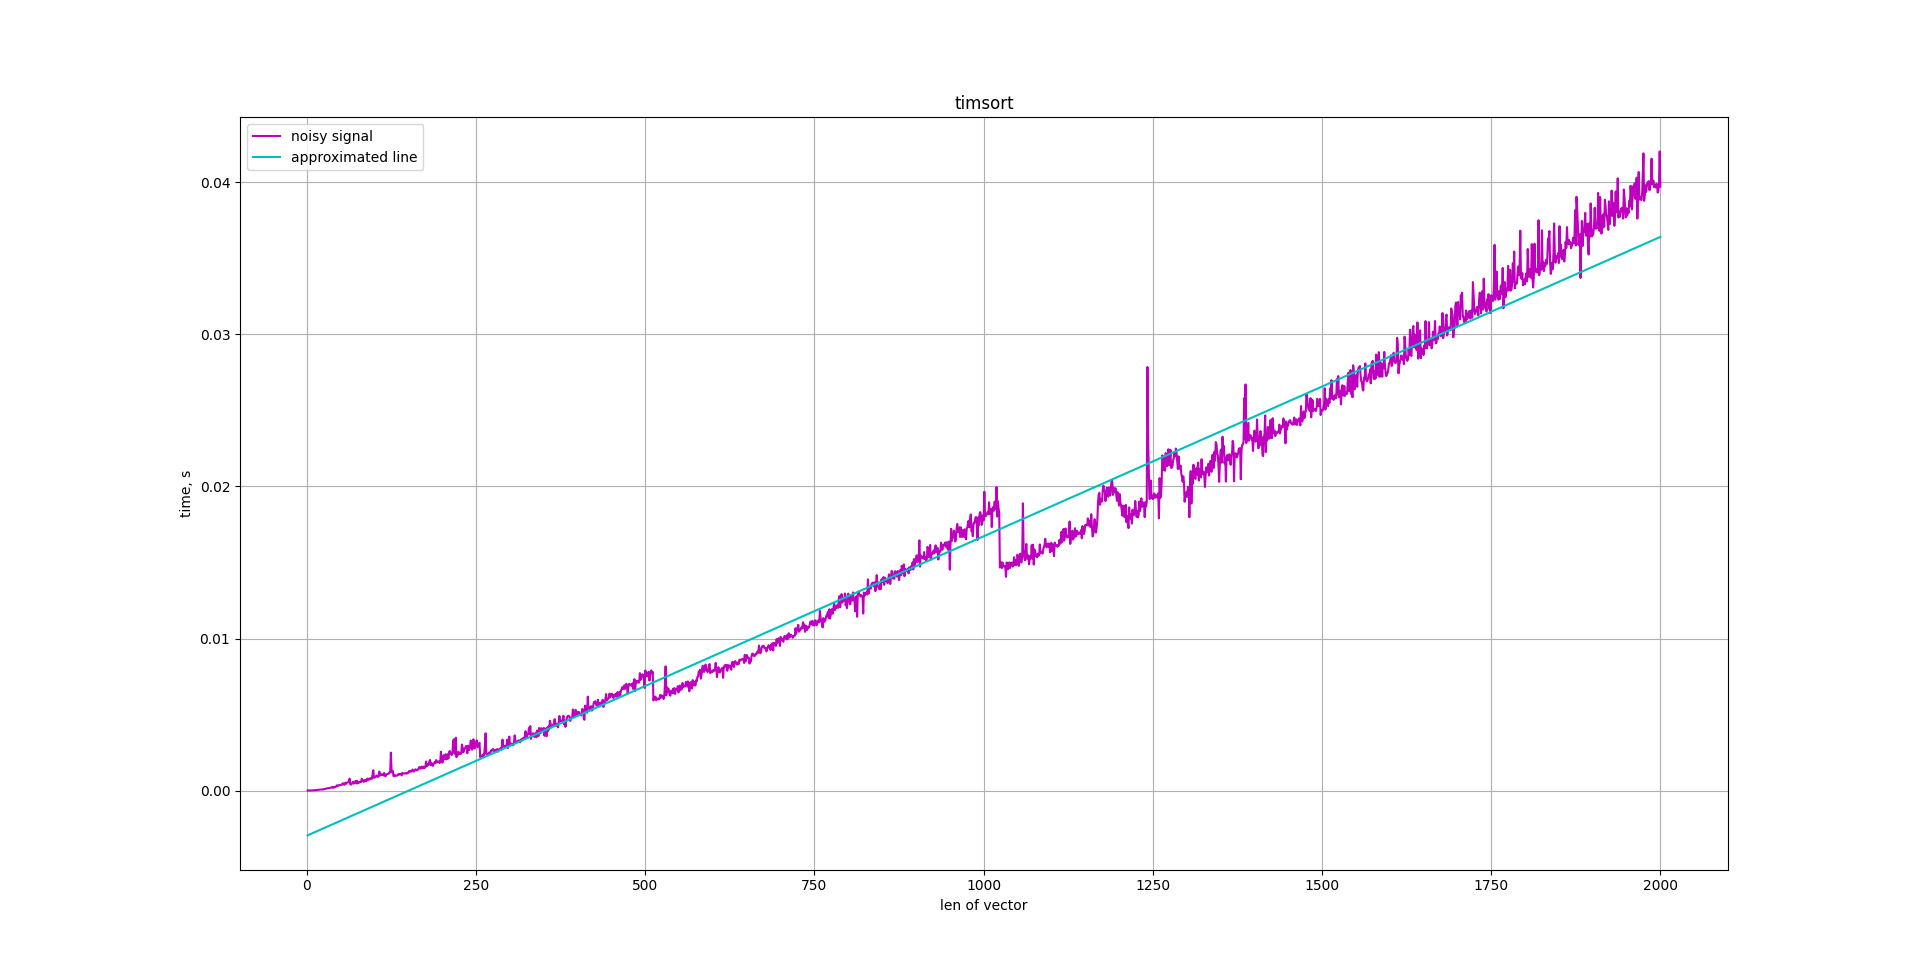
\includegraphics[width=\textwidth]{img/timsort.png}
    \caption{Empirical and theoretical time complexities of an algorithm that implements the TimSort.}
    \label{ris:timsort}
\end{figure}

\paragraph{Matrix product.}

In the \textit{numpy} library of the \textit{Python} programming language, the \textit{matmul} function implements a matrix product using the \textit{Strassen} method and has a theoretical complexity of $O(n^{2.81})$ (Figure \ref{ris:matmul}).

\begin{figure}[H]
    \center
    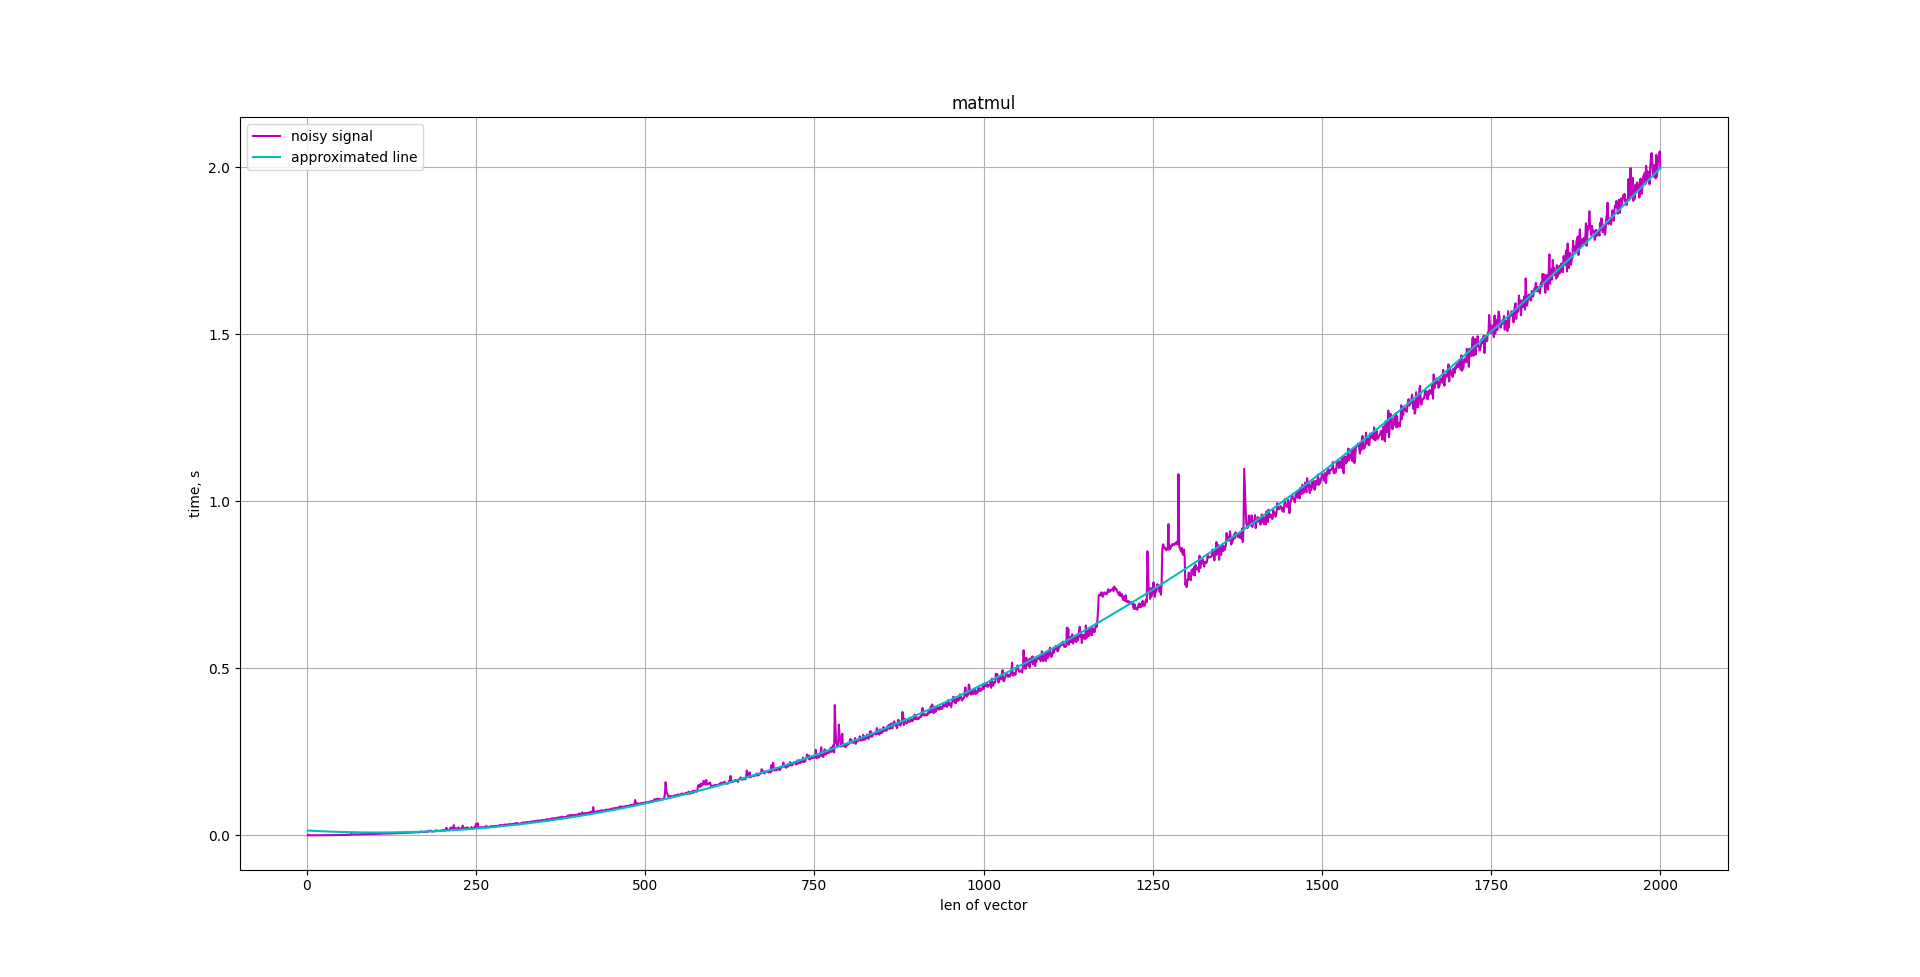
\includegraphics[width=\textwidth]{img/matmul.png}
    \caption{Empirical and theoretical time complexities of an algorithm that implements the matrix product.}
    \label{ris:matmul}
\end{figure}

\subsection{Conclusion}

As a result of this task, algorithms with different time complexity are implemented.
It is shown that the empirical time for the algorithms described above coincides with the theoretical time.
Strategies for implementing algorithms are also described.

\subsection{Appendix}

The source code is located \href{https://github.com/vanSultan/anal_dev_algo/tree/lab_01}{here}: \url{https://github.com/vanSultan/anal_dev_algo/tree/lab_01}.
